% !TEX root = main.tex
\renewcommand{\labelenumi}{\alph{enumi})}
\section*{Tarea 1}
\textbf{2. 
Diseña un AFD $M_{1}$ sobre el alfabeto $\Sigma$ = \{a, b\} que acepte el lenguaje $L_{1}$ tal que la cantidad de b’s
consecutivas es un número par.}

\textbf{1. 
Diseña un AFD $M_{2}$ con $\Sigma$ = \{0, 1\} para el lenguaje $L_{2}$ = \{
$0^{1}1^{1}$ m $|$ n, m $\geq$ 1}


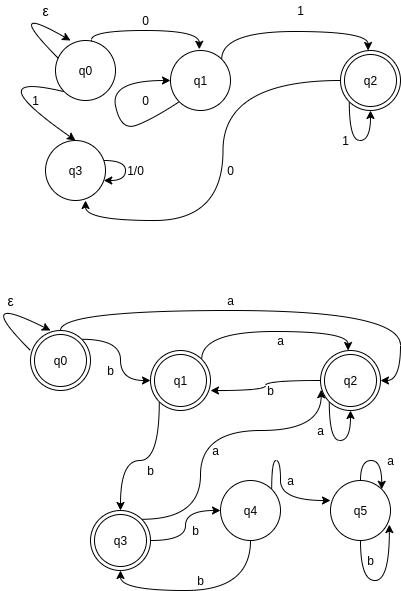
\includegraphics{semanal4.png}